\chapter{Particle-in-Cell Simulations of Enhanced Target Normal Sheath Acceleration} \label{ch:4}

This chapter details the \gls{PIC} simulations I conducted to better understand the double pulse \gls{TNSA} experiments at \gls{LLNL} by Joseph Snyder, Nathaniel Tamminga, and John Morrison in March of 2024. These experiments were done at Titan (which is housed in the \gls{JLF}) for 6 weeks using their earned LaserNetUS \emph{shot time}. I will mostly focus on the simulation aspects of the project, but I include some relevant comparisons to the experiment as needed. 

\section{Background} \label{sec:etnsa_background}

\subsection{Spatially Aligned Pulses} \label{sec:spatialalign}

\begin{figure}
	\centering 
	\includegraphics[width=0.75\linewidth]{planning/images/Markey_Spectrum.PNG}
	\caption{Proton energy spectrum from 1D particle-in-cell simulations depicted for three different temporal delays (including $\Delta t = 0$) from FIG. 3 in Markey et. al. \cite{Markey_2010_PRL}.}
	\label{fig:markey_spectrum}
\end{figure}

As explained in \autoref{sec:tnsa_opt}, there is generally an optimal level of pre-expansion of the target to maximize the \gls{TNSA} proton energies \cite{McKenna_2008_LaPB,Fuchs_2007_PRL}. While the pre-expansion could be due to a low contrast pulse, it could also be due to an artificially injected pre-pulse whose intensity and temporal delay are tunable. Robinson et. al. \cite{Robinson_2007_PPCF} first addresses the idea of using multiple high intensity 40 fs laser pulses with the first being one-tenth to one-quarter of the intensity of the second. They termed this novel two-stage process \emph{multiple pulse sheath acceleration}. This study found a reduction in peak proton energy through numerical simulations, but did find the existence of spectral peaks -- spikes in the energy spectrum at specific energies. A few years later, Markey et. al. \cite{Markey_2010_PRL} examined a similar setup experimentally, varying the temporal separation by 0.75 - 2.5 ps. Interestingly, they found an enhancement in the peak proton energy with a 0.75 ps separation and energy ratio of 0.4:1 between the two pulses. They conducted 1D \gls{PIC} simulations shown in \autoref{fig:markey_spectrum} that verify this as well.

In 2018, Ferri et. al. \cite{Ferri_2018_PoP} re-examines the same question, but uses the same intensity for both pulses. He finds that ultimately, little to no delay is optimal and as the delay gets larger, the enhancement reduces to the single pulse result. He finds the acceleration process can be affected by the second pulse for time delays as long as $\SI{0.6}{\pico \second}$ for $\SI{3}{\micro \meter}$ targets and $\SI{1}{\pico \second}$ for $\SI{6}{\micro \meter}$ targets. 

In a different approach Scott et. al. \cite{Scott_2012_APL} realized that much of the laser light that is reflected is wasted, so a mechanism to re-direct this light back into the target would be desired. They designed a target with a half-cavity foil as seen in \autoref{fig:scott_half_cavity} that will take light reflected off the accelerating foil and re-reflect it back towards the accelerating foil. They find that this can increase the laser to proton energy efficiency by up to $\sim 55 \%$.

\begin{figure}
	\centering 
	\includegraphics[width=0.9\linewidth]{planning/images/scott_half_cavity.PNG}
	\caption{Schematic of the incident laser on the half-cavity target (left) in Scott et. al. \cite{Scott_2012_APL}. The radius of the cavity foil determines the delay ($\tau = 2 r/c$) between the main pulse and the post-pulse (reflected laser light of $\sim 40 \%$ energy of the main pulse).}
	\label{fig:scott_half_cavity}
\end{figure}

\subsection{Spatially and Temporally Aligned Pulses}

Given the results of the previous section \cite{Markey_2010_PRL,Scott_2012_APL,Ferri_2018_PoP} that use short-delay pre or post pulses, Ferri, Siminos and Fulop decided to study how spatially \emph{and} temporally aligned pulses can enhance proton acceleration. They showed that the double pulse setup can result in an almost doubling of the proton energy and five-fold enhancement in the number of protons \cite{Ferri_2019_Nat_Comm} through \gls{PIC} simulations. This phenomena, referred to as double pulse enhanced target normal sheath acceleration, is depicted in \autoref{fig:ferri_dub_pulse} which shows the constructive interference of the fields at the front of the target in the center panel (e) and enhanced \gls{TNSA} fields at the target rear (f).

\begin{figure}
	\centering 
	\includegraphics[width=\linewidth]{planning/images/ferri_dub_pulse.PNG}
	\caption{Geometry of the two pulse scheme as shown in Figure 1 of Ferri et. al. (2019) \cite{Ferri_2019_Nat_Comm}. The single pulse has a total energy of 1.1J at an incidence angle of $\phi=45^\circ$ and is shown through several time snapshots (a-c). In (d-f), the double pulse is shown through those same time snapshots with energies of 0.55 J in each pulse (the 1.55 J is a typo from the original figure). Other parameters include $\tau_\text{fwhm} = \SI{38}{\femto \second}$, thickness = $\SI{3}{\micro \meter}$, material = aluminum, $w_\text{0,fwhm} = \SI{5}{\micro \meter}$, $I_0 = \SI{7e19}{\watt \per \centi \meter \squared}$.}
	\label{fig:ferri_dub_pulse}
\end{figure}
The constructive interference of the electric fields can be understood by considering the electric field of two p-polarized plane waves coming in at angles of incidence $\phi$ and $-\phi$

\begin{align}
	E_{x,1} &= -E_0 \sin(\phi) \sin(k y \sin(\phi) - \omega t + k x \cos(\phi)) \\
	E_{x,2} &= -E_0 \sin(\phi) \sin(k y \sin(\phi) - \omega t - k x \cos(\phi))
\end{align}
Adding these two fields together results in 

\begin{equation}
	E_\text{double} = -2 E_0 \sin(\phi) \sin(k y \sin(\phi) - \omega t) \cos(k x \cos(\phi))
\end{equation}
which has an amplitude of $\lvert E_\text{double} \rvert = 2 E_0 \sin(\phi)$. In contrast, a single pulse with twice the energy (intensity) would only have a $\sqrt{2}$ larger electric field ($\lvert E_\text{single} \rvert = \sqrt{2} E_0 \sin(\phi)$) which explains the enhanced electric fields seen in the bottom row of \autoref{fig:ferri_dub_pulse}. In an ideal situation where 100\% of the laser pulse is reflected, the angles of the two pulses do not need to be equal and opposite -- we will get a standing wave pattern from the constructive interference of the incident wave with its reflection and the same $\sqrt{2}$ field enhancement.  

Unlike the methods described in \autoref{sec:spatialalign} (which see enhanced proton acceleration from a pre-expanded target), double pulse enhanced \gls{TNSA} relies on the presence of an undisturbed target from the vacuum heating mechanism \cite{Brunel_1987_PRL} explained in \autoref{sec:absorption}. Vacuum heating involves the dominance of the electron's quiver motion in the oscillatory electric field in the x-direction, but the magnetic field (which is relevant when $a_0 \gtrsim 1$) may impart a $\vec{v} \times \vec{B}$ Lorentz force (\autoref{eq:lorentz}) that negatively affects the electron acceleration in the x-direction. Brunel even assumes in his original 1987 paper \cite{Brunel_1987_PRL} that we can ignore $\vec{v} \times \vec{B}$ interactions if the laser is split into two equal and opposite angle pulses. Ferri confirms \cite{Ferri_2019_Nat_Comm}, through simulations, that the magnetic field is indeed suppressed in the double pulse case which results in hot electrons accelerated to higher energies. 

\begin{figure}
	\centering 
	\includegraphics[width=\linewidth]{planning/images/ferri_scale_energy.PNG}
	\caption{Double pulse effectiveness in terms of changing preplasma scale length (a) and total laser energy (b,c) from Ferri et. al. (2019) \cite{Ferri_2019_Nat_Comm}.}
	\label{fig:ferri_scale_energy}
\end{figure}

Furthermore, Ferri ran some simulations exploring different preplasma scale lengths $L$ at a fixed energy, and changing the total laser energy for an $L=\SI{0}{\micro \meter}$ target \cite{Ferri_2019_Nat_Comm} which can be seen in \autoref{fig:ferri_scale_energy}. He finds that a higher preplasma scale length generally increases the max proton energy up to a certain scale length of around $L = \SI{0.6}{\micro \meter}$. The enhancement is seen for all scale lengths, but the gap between single and double pulse diminishes for larger scale lengths. In the double pulse case, a more favorable scaling with laser energy is seen for both the hot electron temperature and maximum proton energy ($E_\text{0,tot}$ as opposed to $\sqrt{E_\text{0,tot}}$) when comparing double pulse against single. In addition, Ferri comments that, for pulses with total energy greater than 10 J, the proton layer on the rear side starts to entirely disconnect from the bulk of the target during the acceleration, causing proton energies to saturate and become lower than the expected linear scaling.

\subsection{Other Double Pulse Simulations}
In 2021, double pulse enhanced \gls{TNSA} was again demonstrated through simulations in Rahman et. al. \cite{Rahman_2021_PoP} for a mJ class laser (around 2 orders of magnitude lower energy than the setup in Ferri's work). This mJ class laser is based on the experimental facility at the Wright Patterson Air Force Base (see \autoref{ch:6} for more details) which utilizes a thinner target of $\sim \SI{0.5}{\micro \meter}$. Despite the major difference in laser and target parameters, the findings are similar -- increased hot electron temperature and proton energies with double pulse compared to single pulse. However, Rahman finds that the presence of a preplasma actually \emph{reduces} the maximum proton energy. But, like Ferri et. al., the gap between single and double pulse becomes smaller in the presence of a preplasma.

In 2024, Khan and Saxena \cite{Khan_2024_NJoP} revisit the double pulse scheme but with an applied longitudinal kilo-Tesla level magnetic field. The purpose of the magnetic field is to reduce the divergence of the hot electron beam. This guides the electrons and enhances the \gls{TNSA} process to see a higher maximum cutoff energy in the proton spectrum \cite{Arefiev_2016_NJoP}. In this study, the laser was based off of the experimental set-up at \gls{RAL} with a peak intensity of $\SI{5.5e20}{\watt \per \centi \meter \squared}$ incident on a $\SI{7}{\micro \meter}$ polyethelene target. 

% Preplasma is only on front of target just like titan dub pulse sims

\subsection{Recent Experiments}

Due to multiple simulation studies demonstrating double pulse enhanced \gls{TNSA} \cite{Ferri_2019_Nat_Comm,Rahman_2021_PoP,Khan_2024_NJoP}, experimental confirmation is now needed. Morace et al. \cite{Morace_2019_Nat_Comm} showed that splitting a 270 J beam ($\SI{2.5e18}{\watt \per \centi \meter \squared}$ peak intensity) into multiple ``beamlets'' on Al foil targets enhances the proton energy spectrum. These beamlets (dependent on the incidence angle) induced critical surface density modulations that strongly improved absorption into hot electrons. 

\begin{figure}
	\centering 
	\includegraphics[width=0.75\linewidth]{planning/images/yao_exp_stacks.PNG}
	\caption{Figure 2 from Yao et al. \cite{Yao_2024_MaRaE}. Case 0 shows electron signals from a single pulse. Case 1 shows electron signals from a double pulse with spatial separation $\SI{120}{\micro \meter}$. Case 2 shows electron signals from a double pulse with no spatial separation.}
	\label{fig:yao_exp_stacks}
\end{figure}

Yao et al. \cite{Yao_2024_MaRaE} investigated the double pulse effect by changing the transverse spatial separation between two temporally aligned pulses as shown in \autoref{fig:yao_exp_stacks}. This figure shows two possible beams $\alpha$ and $\beta$ which come in at equal and opposite incidence angles with $\alpha$ angled in the $-\hat{y}$ direction. Comparing\footnote{Note that in \autoref{fig:yao_exp_stacks}(a), the electron energy is recorded along the laser beam axis unlike (b) and (c) which are in the target normal direction. This does not allow us to compare (a) to (b) or (c) directly, but shows that most electrons are getting accelerated along the laser axis.} (b) and (c) shows an enhancement of the double pulse electron energy when the pulses are spatially overlapped. In terms of the protons, case 2 (spatially aligned double pulses) shows a more collimated central small beam which is absent in case 1 (spatially offset double pulses).

\section{Titan Experiment} \label{sec:titan_experiment}

The previous section described prior work that established the theory of double pulse enhanced \gls{TNSA} with relevant experiments discussed. In this section, an experiment to demonstrate this phenomena is described that was conducted by the experimentalists in my research group. The simulations presented here model these experiments. At the time of this writing, this work is not yet published.

The experimental setup involved one (two) $50$ J ($25$ J) $\sim 10^{19} \unit{\watt \per \centi \meter \squared}$ pulse(s) arriving at a $\SI{15}{\micro \meter}$ thick gold target. The Titan laser produces $\tau_\text{FWHM} = 2$ ps pulses of wavelength $\SI{1.053}{\micro \meter}$. The beams can come from one of two \gls{OAP}s. \gls{OAP}1 (\gls{OAP}2) has an incidence angle of $20^\circ$ ($42^\circ$) which can be seen in \autoref{fig:jlf_target_chamber} (the blue beam is from \gls{OAP}1 and the yellow beam is from \gls{OAP}2). These angles of incidence were chosen to differ so that the reflected beams do not travel back to the \gls{OAP}s and cause damage to optimal components. The beam spot size was around $\SI{15}{\micro \meter}$ (in the plane of \autoref{fig:jlf_target_chamber}) and $\SI{8}{\micro \meter}$ (normal to the plane of \autoref{fig:jlf_target_chamber}) for each beam. The proton beams are recorded by three \gls{EPPS}s which are located along each beam axis and in the target normal direction.

\begin{figure}
	\centering
	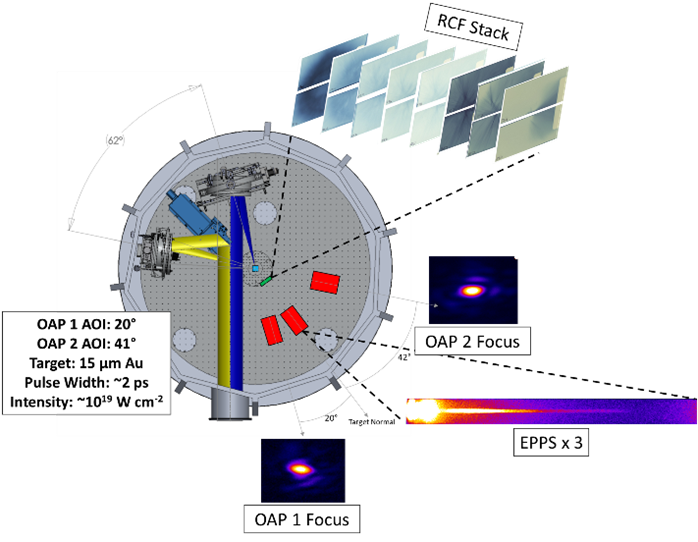
\includegraphics[width=.95\linewidth]{planning/images/titan/target_area_JLF.png}
	\caption{Target chamber schematic showing the split beam configuration at the LaserNet Titan experiment conducted in March of 2024. Two independent off-axis paraboloid mirrors focus each beam onto a 15~$\mu$m Au target. A radio-chromic film stack with aluminum filtering is placed 18.6 cm from ... along the target normal direction. Additionally, three electron positron proton spectrometers are used, one along the target normal direction and one along each beam axis, respectively. This figure was taken from work in preparation by Snyder et al.}
	\label{fig:jlf_target_chamber}
\end{figure}

\subsection{PIC Simulations}

To model this setup, we used 2D(3v) simulations using the EPOCH \gls{PIC} code (version 4.19.0). For simplicity, both pulses had a fixed spot size of $w_\text{FWHM} = \SI{12}{\micro \meter}$ to enable better comparison between the individual pulses. Using a $\SI{2e19}{\watt \per \centi \meter \squared}$ peak intensity, the single pulse would have around 65 J of energy for a sine-squared temporal profile. Accordingly, the double pulse has half the energy and intensity per pulse. We timed the pulses to arrive at the target front around 100 fs into the simulation. Even though the total pulse duration is around $2 \tau_\text{FWHM} = \SI{4}{\pico \second}$, we only run the simulations to 2.2 ps which is more than sufficient to see the highest energy protons produced (within the limited simulation area of tens of microns behind the target). Note that there are two single pulse cases, but the figures below choose \gls{OAP}2 ($41^\circ$) due to higher sheath fields, electron energies, and proton energies observed throughout the simulations (see \autoref{tab:gold_sims}). The gold was initially neutral and allowed to freely ionize through EPOCH's field ionization routine (typically reaching $Z^* = 20$ or $Z^* = 30$ after 1 to 2 ps respectively). No recombination model was used. We employed a ($-\SI{28}{\micro \meter}$, $\SI{42}{\micro \meter}$) square simulation box with $\Delta x = \SI{13.33}{\nano \meter}$ cells and 25 (125) \gls{PPC} for gold (protons).


The $\SI{15}{\micro \meter}$ thick target had a length of $\SI{36}{\micro \meter}$ which can be seen in \autoref{fig:efield_800fs} rotated at a $45^\circ$ angle. The gold target had an initial number density $n_0 = \SI{5.9e28}{\per \meter \cubed}$ with a $\SI{0.5}{\micro \meter}$ layer of protons (of the same density) added to the rear side to enhance the \gls{TNSA} effect. Since the presence of a pre-plasma is known to greatly affect the proton energy spectrum, we also performed simulations where an exponential scale $L_s = \SI{2}{\micro \meter}$ pre-plasma was placed in front of the target of the form: 

\begin{equation}
	n(r) = n_0^* \exp(-r / L_s) \label{eq:exponential_scale_pp}
\end{equation}
where $n_0^* = \SI{5.2e28}{\per \meter \cubed}$ is chosen to be lower than $n_0$ to preserve the same number of particles. The pre-plasma extends from $r_0=0$ (the target front) to $r_\text{cut} = \SI{15.7}{\micro \meter}$ in front of the target. $r_\text{cut}$ corresponds to the location where the gold density would be $n_c / 50$\footnote{This is an arbitrary cutoff which is chosen significantly below the critical density to ensure the laser travels for a significant distance through the pre-plasma. This cutoff was chosen as $n_c / 18$ in Rahman et al. \cite{Rahman_2021_PoP} and $n_c / 100$ in Ferri et al. \cite{Ferri_2019_Nat_Comm}.}. Here, $n_c \approx 10^{27} \unit{\per \meter \cubed}$ is the critical density (from \autoref{eq:criticaldensity}). This pre-plasma will form the critical density surface around $r = \SI{8}{\micro \meter}$ in front of the target which can be seen in the electric fields of \autoref{fig:efield_800fs}(b, d).

\begin{figure}
	\centering
	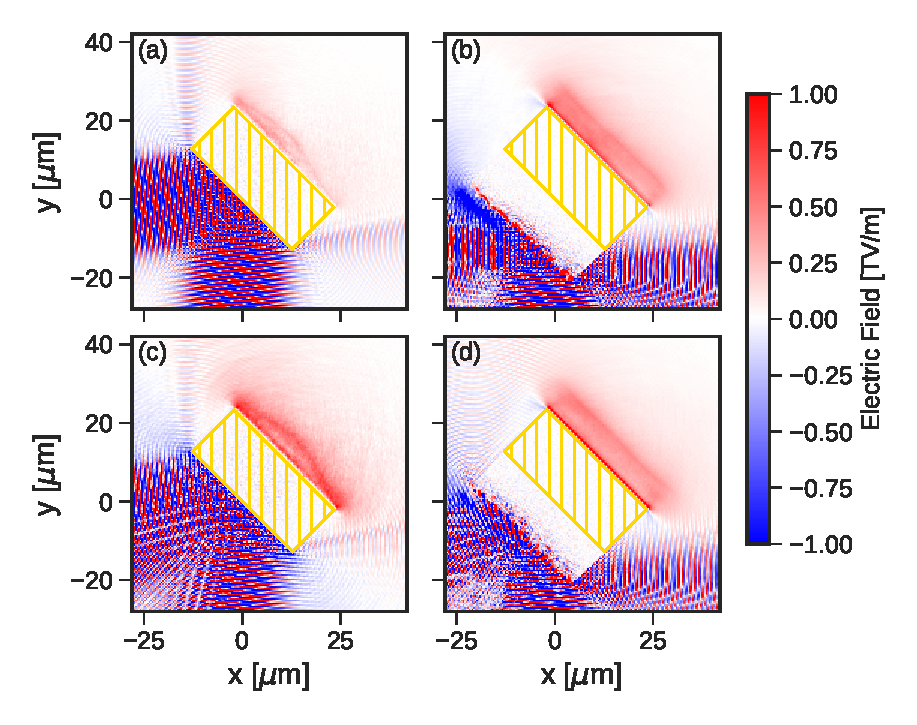
\includegraphics[width=0.9\linewidth]{planning/images/titan/efield_800fs.eps}
	\caption{Electric field in the target normal direction at simulation time of 800 fs for the (a, b) single $41^\circ$ pulse and (c, d) double pulse. In the left column (a, c) the target had a flat density profile at the front, and in the right column (b, d) the target was pre-expanded with an exponentially decaying density in front as described by \autoref{eq:exponential_scale_pp}. These simulations correspond to the first set of four simulations in \autoref{tab:gold_sims}. A hatched gold rectangle is overlaid to visualize the size of the ``flat'' target.}
	\label{fig:efield_800fs}
\end{figure}
From the results of Ferri et al. \cite{Ferri_2019_Nat_Comm}, we would expect the constructive interference of the pulses in front of the target to enhance the electric fields on the back side of the target. This is exactly what we see in \autoref{fig:efield_800fs}(a, c) which is an electric field snapshot 800 fs into the simulation when sheath fields are clearly developed. 

Furthermore, the proton energy enhancement can be seen in \autoref{fig:sim_protons_angular}(a, c) in both the maximum energy and total amount of high energy (i.e. $>$ 1 MeV) protons. This plot bins the protons by both angle (determined from the protons' x and y momentum components) and energy. \autoref{fig:sim_protons_angular}(b, d) shows similar results with the pre-expanded target where the double pulse proton beam focuses to a narrower angular spread with reduced filamentation\footnote{According to dictionary.com a filament is defined as \emph{a very fine thread or threadlike structure}. So, filamentation refers to the threadlike nature of the proton beam (which is not desired).}. Additionally, the number of protons along the target normal direction is higher in the double pulse case as can be seen from the brighter color. 

\begin{figure}
	\centering
	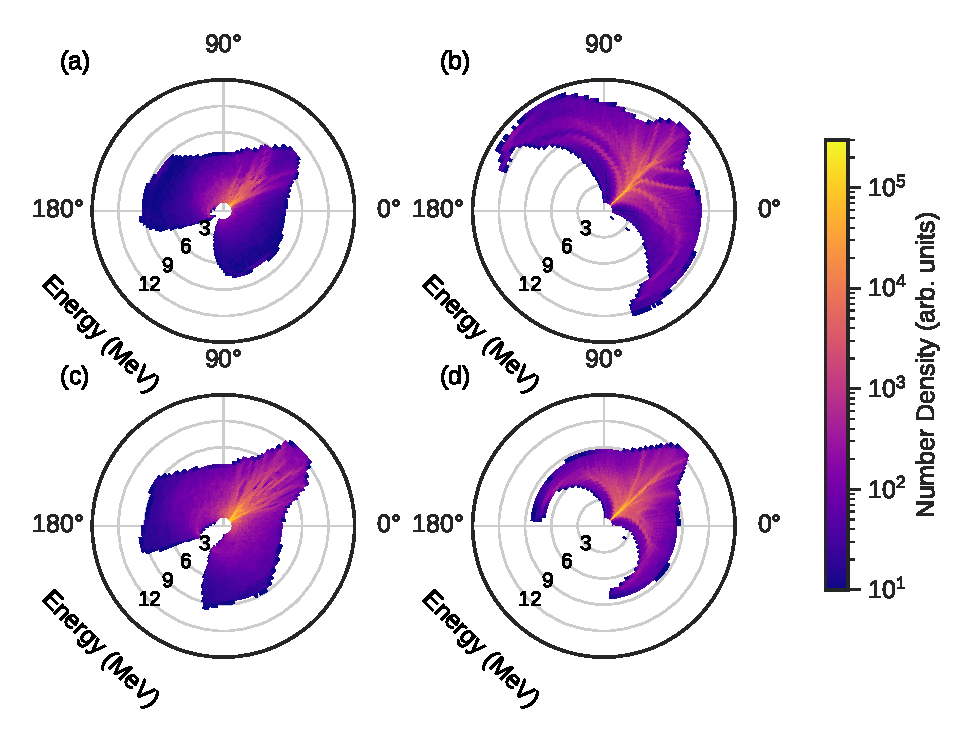
\includegraphics[width=0.9\linewidth]{planning/images/titan/proton_angular_density_2100fs.eps}
	\caption{Proton distribution as a function of angle $\phi = \tan^{-1}(p_y, p_x)$ (where $p$ is the proton momenta) and energy at simulation time of 2100 fs for the same set of simulations in \autoref{fig:efield_800fs}. Only protons with energy greater than 1 MeV are plotted. }
	\label{fig:sim_protons_angular}
\end{figure}

\begin{figure}
	\centering
	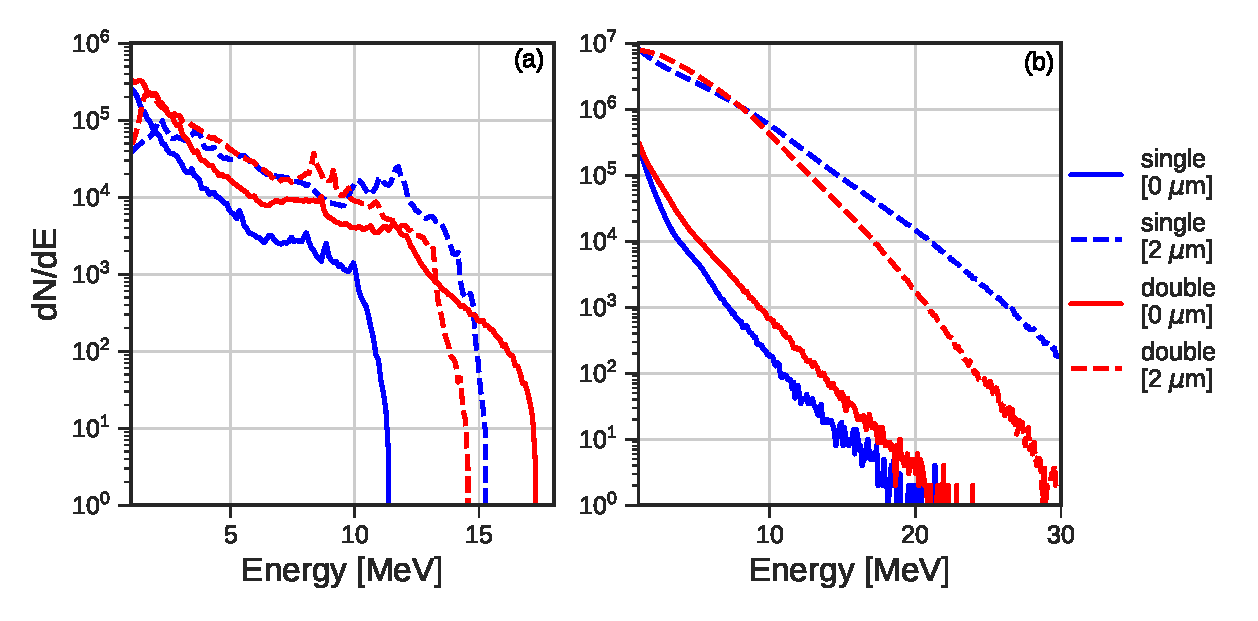
\includegraphics[width=0.9\linewidth]{planning/images/titan/spectrum_2100fs.eps}
	\caption{Spectrum at 2100 fs for (a) protons and (b) electrons for the first set of four simulations in \autoref{tab:gold_sims}. Particles that have left the simulation before 2100 fs are included in the spectrum from their energy at the time of exiting the simulation boundary.}
	\label{fig:sim_spectrum}
\end{figure}

To make these trends clear, the proton energy spectra at 2.1 ps were plotted in \autoref{fig:sim_spectrum} for each of the single and double pulses with and without the $\SI{2}{\micro \meter}$ pre-plasma. We can see (a) that the proton energy spectrum is enhanced in the double pulse scheme for the 0 $\mu$m scale target, but this is not so clear for the case with the 2 $\mu$m scale target. Furthermore, the electron energy spectra (b) shows a clear enhancement in electron energy for both types of targets. 

\begin{figure}
	\centering
	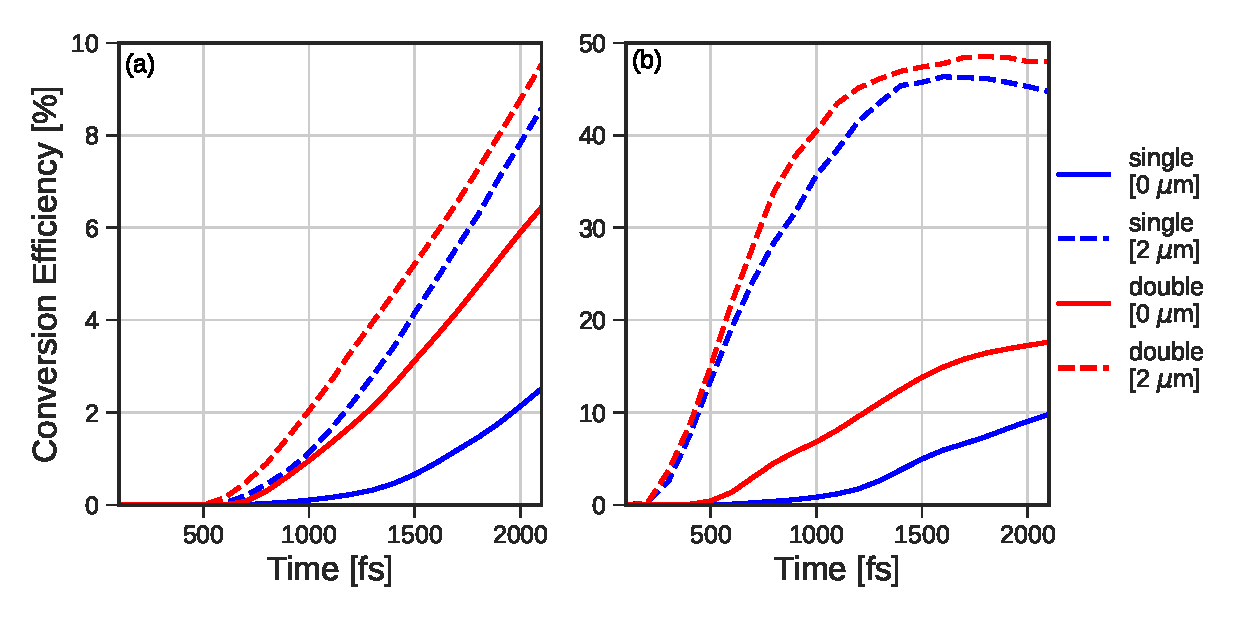
\includegraphics[width=0.9\linewidth]{planning/images/titan/conversion_efficiency.eps}
	\caption{Conversion efficiency of laser energy into greater than 1 MeV (a) protons and (b) electrons for the first set of four simulations in \autoref{tab:gold_sims}.}
	\label{fig:sim_conv_eff}
\end{figure}

Another useful metric is the overall conversion efficiency of laser energy into high energy ($> 1 $ MeV) electrons or protons which is shown in \autoref{fig:sim_conv_eff}. This is computed by dividing the energy in high energy protons or electrons by the total laser energy that entered the simulation at that point in time. Here, both the proton and electron energy enhancement can be seen, although, it bears mentioning that the enhancement is much smaller with the pre-expanded target. 

\renewcommand{\arraystretch}{1.15}
\setlength{\tabcolsep}{0.5em}
\begin{table}
	\centering
	\begin{tabular}{|c|c|c|c|c|p{1.4cm}|c|p{1.4cm}|c|}
		\hline
		\hline
		\textbf{Pulse} & $\pmb{\theta}_i$ & $\mathbf{I}_0$ [$\frac{\text{W}}{\text{cm}^2}$]  & $\mathbf{E}_\text{laser}$ [J] & $\mathbf{L}_p$ [$\mu$m] & $\mathbf{KE}_\text{p,max}$\newline [MeV] & $\pmb{\eta}_\text{p}$ [\%] & $\mathbf{KE}_\text{e,max}$\newline [MeV]& $\pmb{\eta}_{\text{e}}$ [\%] \\
		\hline 
		Single & $20^\circ$ & $2 \times 10^{19}$ & 65 & 0 & 8.5 & 0.5 & 29.8 & 2.0 \\
		\hline
		Single & $41^\circ$ & $2 \times 10^{19}$ & 65 & 0 & 11.35 & 2.5 & 33.48 & 9.8 \\
		Double & $20^\circ, 41^\circ$ & $1 \times 10^{19}$ & 65 & 0 & 17.2 & 6.4 & 27.2 & 17.6 \\
		Single & $41^\circ$ & $2 \times 10^{19}$ & 65 & 2 & 15.4 & 8.6 & 37.6 & 44.7 \\
		Double & $20^\circ, 41^\circ$ & $1 \times 10^{19}$ & 65 & 2 & 14.6 & 9.5 & 31.4 & 48.0 \\
		\hline 
		Single & $41^\circ$ & $1 \times 10^{19}$ & 32.5 & 0 & 9.0 & 1.5 & 14.6 & 5.3 \\
		Double & $20^\circ, 41^\circ$ & $5 \times 10^{18}$ & 32.5 & 0 & 13.9 & 4.4 & 21.3 & 11.4 \\
		Single & $41^\circ$ & $5 \times 10^{18}$ & 16.3 & 0 & 6.4 & 0.6 & 9.7 & 2.0 \\
		Double & $20^\circ, 41^\circ$ & $2.5 \times 10^{18}$ & 16.3 & 0 & 10.6 & 2.5 & 10.1 & 6.0 \\
		\hline
		\hline
	\end{tabular}
	\caption{Summary of Titan Simulations that varied the number of pulses, incidence angle ($\theta_i$), intensity at peak focus ($I_0$), total laser energy ($E_\text{laser}$), and pre-plasma scale length ($L_p$). The maximum kinetic energy $KE_\text{max}$ and conversion efficiency $\eta$ are shown for both electrons (e) and protons (p). The top half of the table includes simulations with $E_\text{laser} = 65$ J which are used in the figures in this section. The bottom half of the table includes simulations with (otherwise identical) lower laser energy.}
	\label{tab:gold_sims}
\end{table}

We also conducted some simulations with either half (32.5 J) or a quarter (16.3 J) of the total laser energy used previously. The maximum kinetic energy and conversion efficiency results for these simulations are also shown in \autoref{tab:gold_sims} which exhibit similar trends to the higher energy simulations.

\subsection{Comparison to Experiment}

The spatial distribution of the protons was recorded with \gls{RCF} which changes color when exposed to certain types of radiation. By stacking the \gls{RCF}, the films can record a proton dose calibrated to higher energies for films further along in the stack. We can see these results in \autoref{fig:exp_rcf} which show spatial proton distributions for a selection of energies. Each row is a different shot with total energy at or slightly below 50 J. These images show that both the $20^\circ$ and $41^\circ$ single pulses have a proton distribution that is not centered in the target normal direction (which lies along the hole in the center). The $20^\circ$ pulse records higher doses on the right side because that is where the laser axis of OAP1 points (similar for the $41^\circ$). The double pulse sees protons that have a more even distribution throughout the entire \gls{RCF} square that appears to have its highest dose right in the center.

\begin{figure}
	\centering
	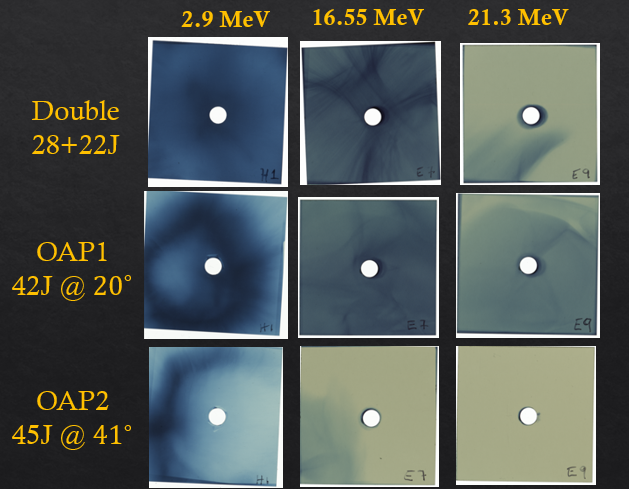
\includegraphics[width=0.9\linewidth]{planning/images/titan/rcf.png}
	\caption{Three slices of radio-chromic film stacks that measure proton doses at 2.9, 16.55, and 21.3 MeV for 3 different pulse arrangments. A darker blue color indicates a higher proton dose at a given spatial location. For reference, the stacks are $2 \times 2$ inch squares that are placed 18.6 cm behind the target.}
	\label{fig:exp_rcf}
\end{figure}

In \autoref{fig:exp_rcf}, I have focused on only three shots and three energies, but all of the shots for which the pulses had a nominal 50 J of energy are plotted in \autoref{fig:50JRCF}. The total dose is plotted on the y-axis for each shot and for each energy that the \gls{RCF} stacks are calibrated to. These show that the double pulse arrangement (blue circles) yields a higher dose in the higher energy stacks (i.e. in the range 13-23 MeV). 

\begin{figure}
	\centering
	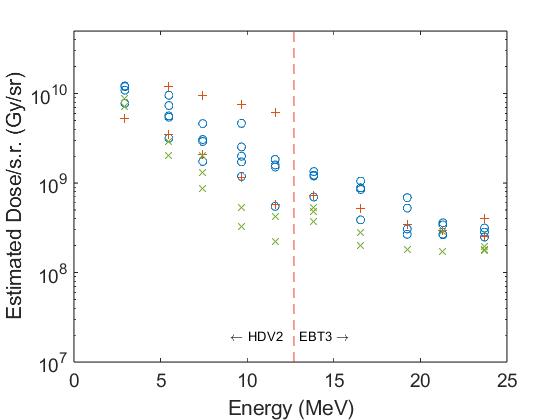
\includegraphics[width=0.75\linewidth]{planning/images/titan/50JRCFcompNew.png}
	\caption{The radio-chromic film total estimated dose for all 50J shots. The blue circles indicate when both beams were used, while the orange + and green x markers indicate when beams 1 and 2 were used, respectively. These results are not calibrated, they are estimated from a calibration in Chris Willis' dissertation. This is why the y axis is estimated in units of Gy/sr. The implementation of sr allows for comparison of different size RCF stacks.}
	\label{fig:50JRCF}
\end{figure}

\section{Discussion}

In \autoref{sec:etnsa_background}, I reviewed the theoretical and experimental background behind the double pulse enhanced target normal sheath acceleration mechanism. This enhancement is largely due to two factors. First, the constructive interference of both pulses is capable of producing $\sqrt{2}$ times higher peak fields at the front of the target using the same total laser energy. The higher electric fields at the target front is directly related to both the hot electron generation and the maximum proton energy. Second, the symmetry of using two pulses at opposite incidence can mitigate unwanted magnetic field deflections that help reduce filamentation and keep proton beams centered along the target normal direction. 

Then, in \autoref{sec:titan_experiment}, I showed results of particle-in-cell simulations that show a clear enhancement in both the maximum proton energy and conversion efficiency of laser energy into high energy protons. When adding an exponential scale pre-plasma to the front of the target, these enhancements diminished. However, the double pulse simulations still demonstrated a more focused proton beam along the target normal direction with reduced filamentation. On the experimental side, the double pulse showed a slightly higher total proton dose and comparable or slightly lower maximum proton energy than the single pulse case which is in agreement with the simulation results in the presence of a pre-plasma.

In conjunction, the results of experiment and simulations suggest that picosecond lasers like Titan can demonstrate double pulse enhanced proton acceleration by both accelerating more protons and collimating the protons in the target normal direction. The maximum proton energy enhancement seems to be most pronounced for an undisturbed target with a sharp density profile which is supported by prior work from this group \cite{Rahman_2021_PoP}. The experimental results most likely matched the simulation results with a pre-plasma due to an imperfect temporal pulse alignment. In the experiments when looking at results with different temporal timing\footnote{Not shown in this work, but will be included in the publication}, the maximum proton energies were seen at both 0 and -2 picosecond delays. Since the experiment was only able to temporally resolve the timing of the pulses down to 2 picoseconds, this means that the temporal alignment may have been off on the order of a picosecond. As mentioned in \autoref{sec:etnsa_background}, this delay would cause pre-mature expansion of the target that may disturb the flat density profile needed for optimal target normal sheath acceleration. 

While it may be difficult to time both pulses to arrive at the target within femtosecond resolution, the double pulse setup is still capable of increasing proton counts and reducing a proton beam's angular divergence. The double pulse setup can be extended to multiple pulses (like \cite{Morace_2019_Nat_Comm}) for a potentially even greater effect. Since there is a significant amount of time and money that goes into upgrading existing laser facilities, the double (or multiple) pulse approach is a great tool for scientists to see enhanced proton/ion generation when constrained by laser energy from current technology.